%% Copernicus Publications Manuscript Preparation Template for LaTeX Submissions
%% ---------------------------------
%% This template should be used for copernicus.cls
%% The class file and some style files are bundled in the Copernicus Latex Package, which can be downloaded from the different journal webpages.
%% For further assistance please contact Copernicus Publications at: production@copernicus.org
%% https://publications.copernicus.org/for_authors/manuscript_preparation.html


%% Please use the following documentclass and journal abbreviations for discussion papers and final revised papers.

%% 2-column papers and discussion papers
\documentclass[essd, manuscript]{copernicus}

\usepackage[default, scale=0.95]{opensans}
\usepackage[section]{placeins}
\usepackage{amsmath}
\usepackage[final]{pdfpages}
\usepackage{lscape}
\usepackage{longtable}
\usepackage{booktabs}

%% Journal abbreviations (please use the same for discussion papers and final revised papers)


% Advances in Geosciences (adgeo)
% Advances in Radio Science (ars)
% Advances in Science and Research (asr)
% Advances in Statistical Climatology, Meteorology and Oceanography (ascmo)
% Annales Geophysicae (angeo)
% Archives Animal Breeding (aab)
% ASTRA Proceedings (ap)
% Atmospheric Chemistry and Physics (acp)
% Atmospheric Measurement Techniques (amt)
% Biogeosciences (bg)
% Climate of the Past (cp)
% DEUQUA Special Publications (deuquasp)
% Drinking Water Engineering and Science (dwes)
% Earth Surface Dynamics (esurf)
% Earth System Dynamics (esd)
% Earth System Science Data (essd)
% E&G Quaternary Science Journal (egqsj)
% Fossil Record (fr)
% Geochronology (gchron)
% Geographica Helvetica (gh)
% Geoscience Communication (gc)
% Geoscientific Instrumentation, Methods and Data Systems (gi)
% Geoscientific Model Development (gmd)
% History of Geo- and Space Sciences (hgss)
% Hydrology and Earth System Sciences (hess)
% Journal of Micropalaeontology (jm)
% Journal of Sensors and Sensor Systems (jsss)
% Mechanical Sciences (ms)
% Natural Hazards and Earth System Sciences (nhess)
% Nonlinear Processes in Geophysics (npg)
% Ocean Science (os)
% Primate Biology (pb)
% Proceedings of the International Association of Hydrological Sciences (piahs)
% Scientific Drilling (sd)
% SOIL (soil)
% Solid Earth (se)
% The Cryosphere (tc)
% Web Ecology (we)
% Wind Energy Science (wes)


%% \usepackage commands included in the copernicus.cls:
%\usepackage[german, english]{babel}
%\usepackage{tabularx}
%\usepackage{cancel}
%\usepackage{multirow}
%\usepackage{supertabular}
%\usepackage{algorithmic}
%\usepackage{algorithm}
%\usepackage{amsthm}
%\usepackage{float}
%\usepackage{subfig}
%\usepackage{rotating}


\usepackage{hyperref}

\begin{document}

\title{The Malina oceanographic expedition: How do changes in ice cover, permafrost and UV radiation impact on biodiversity and biogeochemical fluxes in the Arctic Ocean?}

% \Author[affil]{given_name}{surname}

\Author[1]{Philippe}{Massicotte}
\Author[2,3]{Rainer}{Amon}
\Author[4,5]{David}{Antoine}
\Author[6]{Philippe}{Archambault}
\Author[7,8,9]{Sergio}{Balzano}
\Author[10]{Simon}{Bélanger}
\Author[11,12]{Ronald}{Benner}
\Author[7]{Dominique}{Boeuf}
\Author[5]{Annick}{Bricaud}
\Author[1]{Flavienne}{Bruyant}
\Author[13]{Gwenaëlle}{Chaillou}
\Author[14]{Malik}{Chami}
\Author[15]{Bruno}{Charrière}
\Author[16]{Jingan}{Chen}
\Author[5]{Hervé}{Claustre}
\Author[1]{Pierre}{Coupel}
\Author[15]{Nicole}{Delsaut}
\Author[5]{David}{Doxaran}
\Author[17]{Jens}{Ehn}
\Author[18]{Cédric}{Fichot}
\Author[1]{Marie-Hélène}{Forget}
\Author[19]{Pingqing}{Fu}
\Author[1]{Jonathan}{Gagnon}
\Author[20]{Nicole}{Garcia}
\Author[21]{Beat}{Gasser}
\Author[22]{Jean-François}{Ghiglione}
\Author[5]{Gaby}{Gorsky}
\Author[13]{Michel}{Gosselin}
\Author[23]{Priscillia}{Gourvil}
\Author[24]{Yves}{Gratton}
\Author[13]{Pascal}{Guillot}
\Author[25]{Hermann J.}{Heipieper}
\Author[15]{Serge}{Heussner}
\Author[26]{Stan}{Hooker}
\Author[27]{Yannick}{Huot}
\Author[28]{Violaine}{Jacq}
\Author[7]{Christian}{Jeanthon}
\Author[29]{Wade}{Jeffrey}
\Author[22]{Fabien}{Joux}
\Author[30]{Kimitaka}{Kawamura}
\Author[31]{Bruno}{Lansard}
\Author[5]{Edouard}{Leymarie}
\Author[32]{Heike}{Link}
\Author[1]{Connie}{Lovejoy}
\Author[1,33]{Claudie}{Marec}
\Author[7]{Dominique}{Marie}
\Author[1]{Johannie}{Martin}
\Author[34]{Philippe}{Martinez}
\Author[1,35]{Guillaume}{Massé}
\Author[1]{Atsushi}{Matsuoka}
\Author[5,36]{Alexandre}{Mignot}
\Author[37]{William L.}{Miller}
\Author[21]{Juan-Carlos}{Miquel}
\Author[38]{Alfonso}{Mucci}
\Author[39]{Kaori}{Ono}
\Author[22]{Eva}{Ortega}
\Author[20]{Christos}{Panagiotopoulos}
\Author[17]{Tim}{Papakyriakou}
\Author[20]{Julien}{Para}
\Author[5]{Marc}{Picheral}
\Author[40,41]{Dieter}{Piepenburg}
\Author[5]{Louis}{Prieur}
\Author[20]{Patrick}{Raimbault}
\Author[5]{Joséphine}{Ras}
\Author[42]{Rick A.}{Reynolds}
\Author[13]{André}{Rochon}
\Author[20]{Jean-François}{Rontani}
\Author[43]{Catherine}{Schmechtig}
\Author[34]{Sabine}{Schmidt}
\Author[20]{Richard}{Sempéré}
\Author[11,44]{Yuan}{Shen}
\Author[45,46]{Guisheng}{Song}
\Author[42]{Dariusz}{Stramski}
\Author[47]{Dave}{Stroud G.}
\Author[39]{Eri}{Tachibana}
\Author[5]{Alexandre}{Thirouard}
\Author[21]{Imma}{Tolosa}
\Author[1]{Jean-Éric}{Tremblay}
\Author[48]{Mickael}{Vaïtilingom}
\Author[7,49]{Daniel}{Vaulot}
\Author[20]{Frédéric}{Vaultier}
\Author[50]{John K.}{Volkman}
\Author[51]{Jorien E.}{Vonk}
\Author[52,53]{Vanessa}{Wright}
\Author[13]{Huixiang}{Xie}
\Author[42,54,55]{Guangming}{Zheng}
\Author[1]{Marcel}{Babin}
    
\affil[1]{Takuvik Joint International Laboratory / UMI 3376, ULAVAL (Canada) - CNRS (France), Université Laval, Québec, QC, Canada}
\affil[2]{Department of Marine and Coastal Environmental Science, Texas A\&M University Galveston Campus, Galveston, Texas, 77553, USA}
\affil[3]{Department of Oceanography, Texas A\&M University, College Station, Texas, 77843, USA}
\affil[4]{Remote Sensing and Satellite Research Group, School of Earth and Planetary Sciences, Curtin University, Perth, WA 6845, Australia}
\affil[5]{Sorbonne Université, CNRS, Laboratoire d’Océanographie de Villefranche (LOV) / UMR 7093, F-06230 Villefranche-sur-Mer, France}
\affil[6]{ArcticNet, Québec-Océan, Takuvik Joint International Laboratory / UMI 3376, ULAVAL (Canada) - CNRS (France), Université Laval, Québec, QC, Canada}
\affil[7]{Sorbonne Université, CNRS, Station Biologique de Roscoff - Adaptation et Diversité en Milieu Marin / UMR 7144, 29680 Roscoff, France}
\affil[8]{Present address: Stazione Zoologica Anton Dohrn Napoli (SZN), Naples, Italy}
\affil[9]{NIOZ Royal Netherlands Institute for Sea Research, Den Burg, Netherlands}
\affil[10]{Département de Biologie, Chimie et Géographie (groupes BORÉAS et Québec-Océan), Université du Québec à Rimouski, Rimouski, QC, Canada}
\affil[11]{School of the Earth, Ocean and Environment, University of South Carolina, Columbia, South Carolina, 29208, USA}
\affil[12]{Department of Biological Sciences, University of South Carolina, Columbia, South Carolina, 29208, USA}
\affil[13]{Québec-Océan, Institut des sciences de la mer de Rimouski (ISMER), Université du Québec à Rimouski, Rimouski, QC, Canada}
\affil[14]{Sorbonne Université, CNRS, Laboratoire Atmosphères Milieux Observations Spatiales (LATMOS) / UMR 8190, Boulevard de l’Observatoire, CS 34229, 06304 Nice Cedex, France}
\affil[15]{Université de Perpignan Via Domitia (UPVD), CNRS, Centre de Formation et de Recherche sur les Environnements Méditerranéens (CEFREM) / UMR 5110, 52 Avenue Paul Alduy, 66860 Perpignan Cedex, France}
\affil[16]{SKLEG, Institute of Geochemistry, Chinese Academy of Sciences, 99 West Lincheng Road, Guiyang, Guizhou 550081, P.R. China}
\affil[17]{Centre for Earth Observation Science, Department of Environment and Geography, University of Manitoba, Winnipeg, MB, Canada}
\affil[18]{Department of Earth and Environment, Boston University, Boston, Massachusetts, 02215, USA}
\affil[19]{Institute of Surface-Earth System Science, Tianjin University, Tianjin, China}
\affil[20]{Aix Marseille Université, Université de Toulon, CNRS, IRD, Mediterranean Institute of Oceanography (MIO) UM 110, 13288 Marseille, France}
\affil[21]{International Atomic Energy Agency (IAEA) / Environment Laboratories, MC98000, Monaco, Monaco}
\affil[22]{Sorbonne Université, CNRS, Laboratoire d’Océanographie Microbienne (LOMIC) / UMR 7621, Observatoire Océanologique de Banyuls, France}
\affil[23]{Sorbonne Université, CNRS, Station Biologique de Roscoff - Centre de recherche et d'enseignement en biologie et écologie marines / FR2424, 29680 Roscoff, France}
\affil[24]{Institut national de la recherche scientifique - Centre Eau Terre Environnement (INRS-ETE), Québec, QC, Canada}
\affil[25]{Department of Environmental Biotechnology Permoserstraße 15 D-04318 Leipzig, Germany}
\affil[26]{Ocean Ecology Laboratory, NASA Goddard Space Flight Center, Greenbelt, MD, United States}
\affil[27]{Département de géomatique appliquée, Université de Sherbrooke, Sherbrooke, QC, Canada}
\affil[28]{Sorbonne Université, CNRS, Laboratoire d'océanographie et du climat : expérimentations et approches numériques (LOCEAN) - UMR 7159, 4, place Jussieu, 75252 PARIS Cedex 05, France}
\affil[29]{Center for Environmental Diagnostics \& Bioremediation, Universty of West Florida, 11000 University Parkway, Pensacola, FL 32514 USA}
\affil[30]{Chubu Institute for Advanced Studies, Chubu University, Kasugai, Japan}
\affil[31]{IPSL and Université Paris-Saclay, CEA-CNRS-UVSQ, Laboratoire des Sciences du Climat et de l’Environnement (LSCE) / UMR 8212, 91190 Gif-sur-Yvette, France}
\affil[32]{Department Maritime Systems, University of Rostock, 18059 Rostock, Germany}
\affil[33]{Université de Bretagne Occidentale - UBO, CNRS, IRD, Institut Universitaire Européen de la Mer (IUEM) / UMS 3113,  29280 Plouzané, France}
\affil[34]{Université de Bordeaux, CNRS, OASU, Environnements et Paléoenvironnements Océaniques et Continentaux (EPOC) / UMR 5805, F-33615 Pessac, France}
\affil[35]{Station Marine de Concarneau, MNHN-CNRS-UPMC-IRD, Laboratoire d'océanographie et du climat : expérimentations et approches numériques (LOCEAN) / UMR 7159, 29900 Concarneau, France}
\affil[36]{Mercator Ocean International, Parc Technologique du Canal, 8-10 rue Hermès – Bâtiment C, 31520 Ramonville Saint-Agne, France}
\affil[37]{Department of Marine Sciences, University of Georgia, 325 Sanford Dive, Athens, GA 30602}
\affil[38]{GEOTOP and Department of Earth and Planetary Sciences, McGill University, Montréal, QC, Canada}
\affil[39]{Institute of Low Temperature Science, Hokkaido University, Sapporo, 060-0819, Japan}
\affil[40]{Alfred Wegener Institute, Helmholtz Centre for Polar and Marine Research, Am Handelshafen 12, 27570 Bremerhaven, Germany}
\affil[41]{Helmholtz Institute for Functional Marine Biodiversity at the University of Oldenburg, Ammerländer Heerstraße 231, 26129 Oldenburg, Germany}
\affil[42]{Marine Physical Laboratory, Scripps Institution of Oceanography, University of California San Diego, La Jolla, CA, USA}
\affil[43]{Sorbonne Université, CNRS, Ecce Terra Observatoire des Sciences de l'Univers (OSU)  - UMS 3455,  4, Place Jussieu 75252 Paris Cedex 05, France}
\affil[44]{State Key Laboratory of Marine Environmental Science, College of Ocean and Earth Sciences, Xiamen University, Xiamen, Fujian, P. R. China}
\affil[45]{Institut des sciences de la mer de Rimouski (ISMER), Université du Québec à Rimouski, Rimouski, QC, Canada}
\affil[46]{School of Marine Science and Technology, Tianjin University, Tianjin, 300072, China}
\affil[47]{Department of Physics, Ohio State University, Columbus, Ohio 43210, USA}
\affil[48]{Université des Antilles Pointe-à-Pitre, Laboratoire de Recherche en Géosciences et Energies (LARGE) / EA 4539, Guadeloupe, France}
\affil[49]{Asian School of the Environment, Nanyang Techonological University, Singapore}
\affil[50]{CSIRO Marine and Atmospheric Research and CSIRO Wealth from Oceans Nationa lResearch Flagship, GPO Box 1538, Hobart, Tasmania 7001, Australia}
\affil[51]{Department of Earth Sciences, Vrije Universiteit Amsterdam, The Netherlands}
\affil[52]{NASA Goddard Space Flight Center, Calibration and Validation Office, Science Systems and Applications Inc., Greenbelt, MD, USA}
\affil[53]{Center for Marine and Environmental Studies, University of the Virgin Islands, St. Thomas, VI, USA}
\affil[54]{NOAA/NESDIS Center for Satellite Applications and Research, 5830 University Research Court, College Park, MD 20740, USA}
\affil[55]{Earth System Science Interdisciplinary Center, University of Maryland Research Park, 5825 University Research Court, College Park, MD 20740, USA}

%% The [] brackets identify the author with the corresponding affiliation. 1, 2, 3, etc. should be inserted.

\runningtitle{The MALINA oceanographic expedition: an overview}

\runningauthor{Massicotte et al.}

\correspondence{Marcel Babin (marcel.babin@takuvik.ulaval.ca)}

\received{}
\pubdiscuss{} %% only important for two-stage journals
\revised{}
\accepted{}
\published{}

%% These dates will be inserted by Copernicus Publications during the typesetting process.

\firstpage{1}

\maketitle

\begin{abstract}
    
\end{abstract}

%\copyrightstatement{TEXT}

\introduction  %% \introduction[modified heading if necessary]

\section{Study area, environmental conditions and sampling strategy}

\subsection{Study area and environmental conditions}

\subsubsection{CTD and rosette deployments}

\newpage

\section{Figures}

\begin{figure}[H]
    \centering
    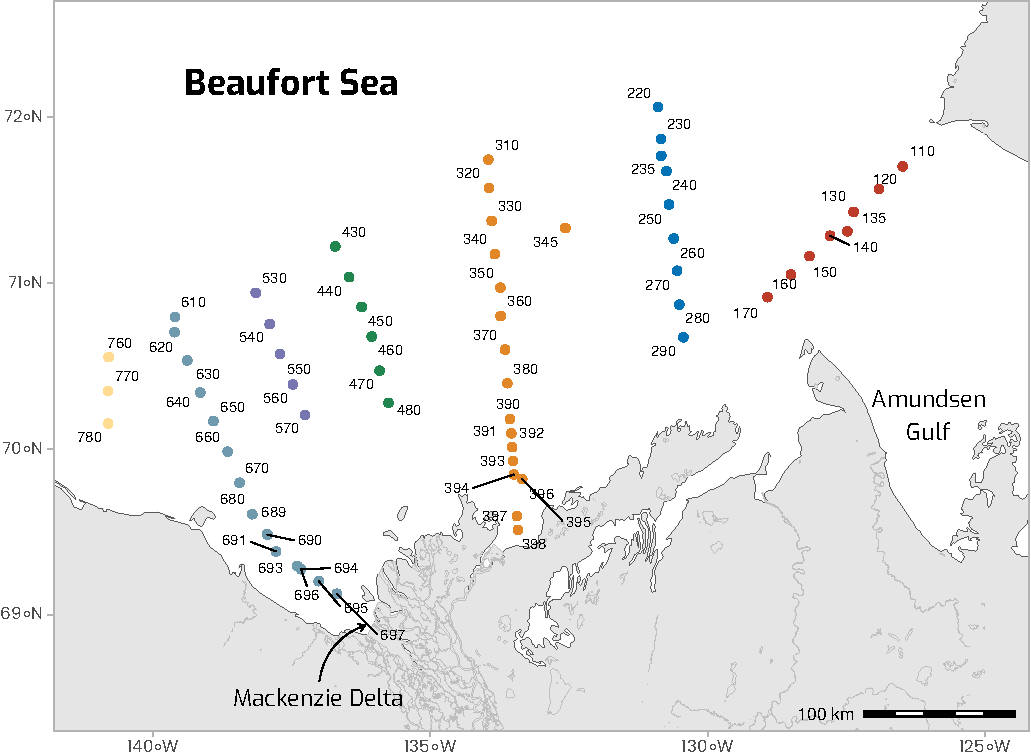
\includegraphics[scale = 1]{../../../graphs/fig01.pdf}
    \caption{(\textbf{A}) Localizations of the sampling sites visited during the MALINA 2009 campaign. The colors of the dots represent the seven transects visited during the mission. (\textbf{B}) Bathymetric profiles for transects 600 and 300. Bathymetric data from GEBCO (https://download.gebco.net/).}
\end{figure}

\clearpage

\begin{figure}[H]
    \centering
    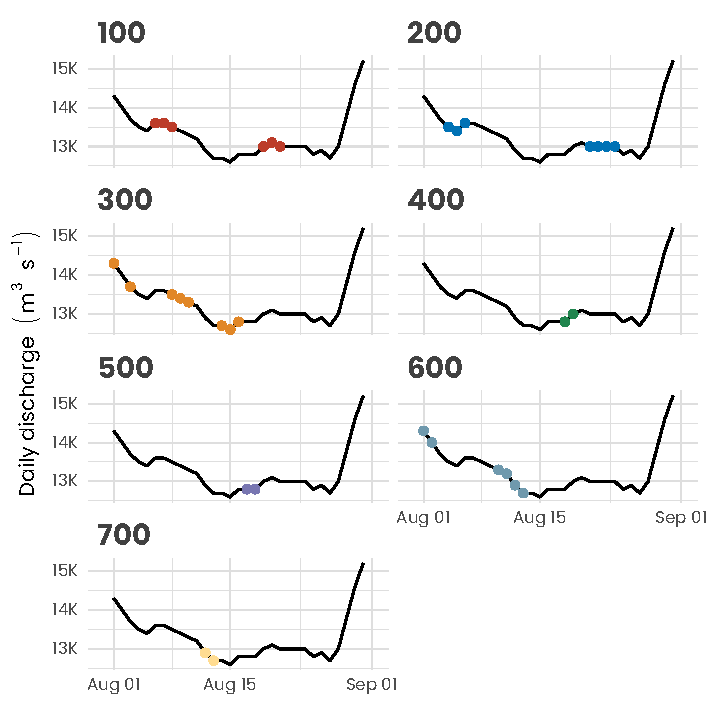
\includegraphics[scale = 1]{../../../graphs/fig02.pdf}
    \caption{(\textbf{A}) Daily discharge of the Mackenzie River at the Arctic Red River junction (station 10LC014). The black line corresponds to the 2009 discharge whereas the coloured segment identifies the period of the MALINA campaign. The shaded area is the mean discharge calculated between 1972 and 2016. Discharge data from the Government of Canada (https://wateroffice.ec.gc.ca/search/historical\_e.html). (\textbf{B}) Hourly air temperature recorded from the Amundsen's foredeck meteorological tower during the campaign.}
\end{figure}

\clearpage

\begin{figure}[H]
    \centering
    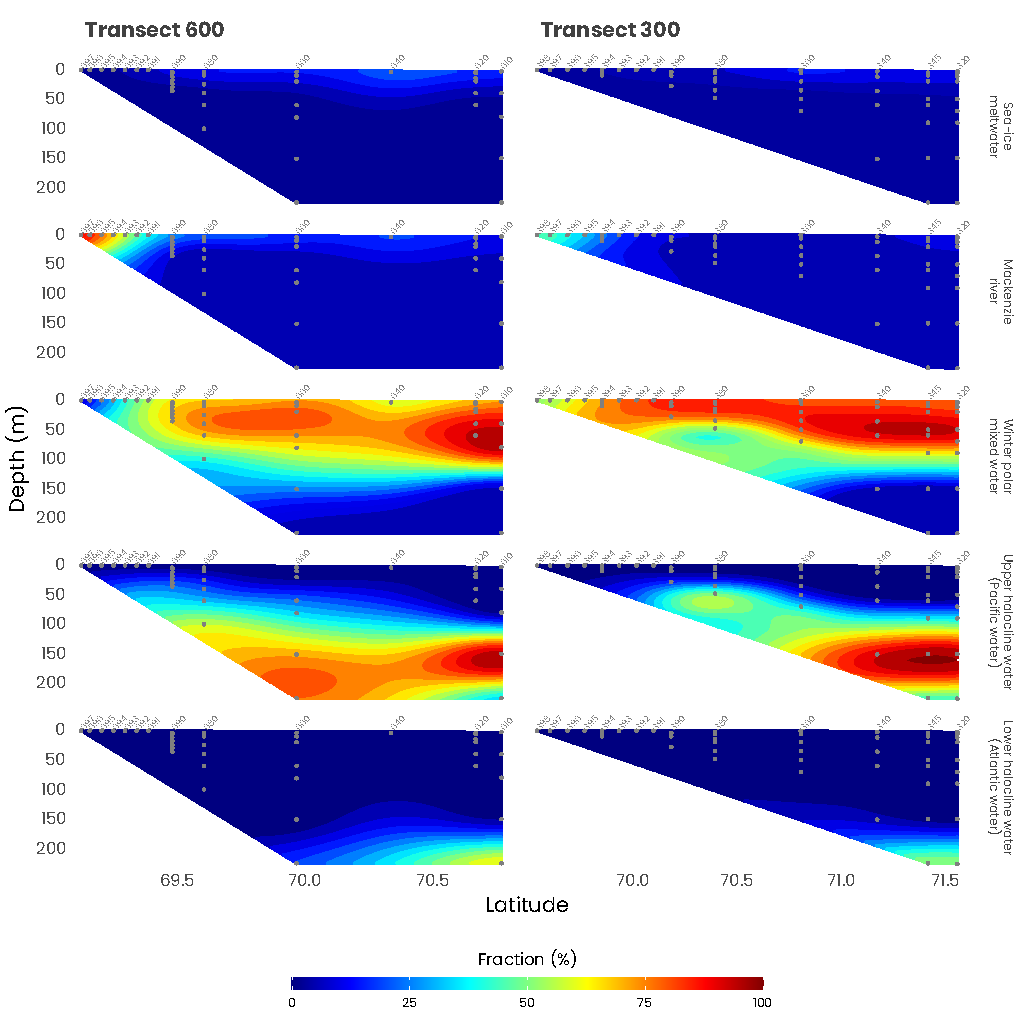
\includegraphics[scale = 1]{../../../graphs/fig03.pdf}
    \caption{Distribution of source water types along transects 600 and 300 (see Fig. 1). Station numbers are identified in light gray on top of each panel.}
\end{figure}

\clearpage

\begin{figure}[H]
    \centering
    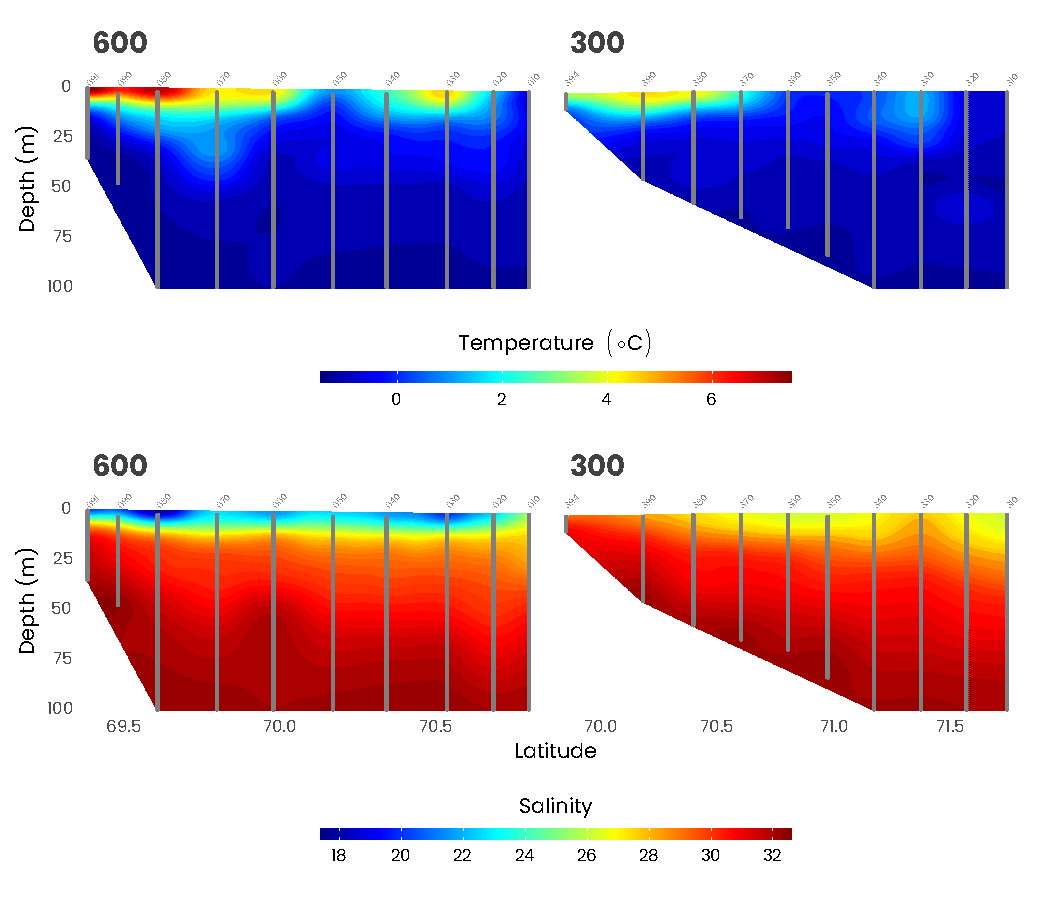
\includegraphics[scale = 1]{../../../graphs/fig04.pdf}
    \caption{Cross-sections of temperature (\textbf{A}) and salinity (\textbf{B}) measured by the CTD (gray dots) along transects 600 and 300. Station numbers are identified in light gray on top of each panel.}
\end{figure}

\clearpage

\begin{figure}[H]
    \centering
    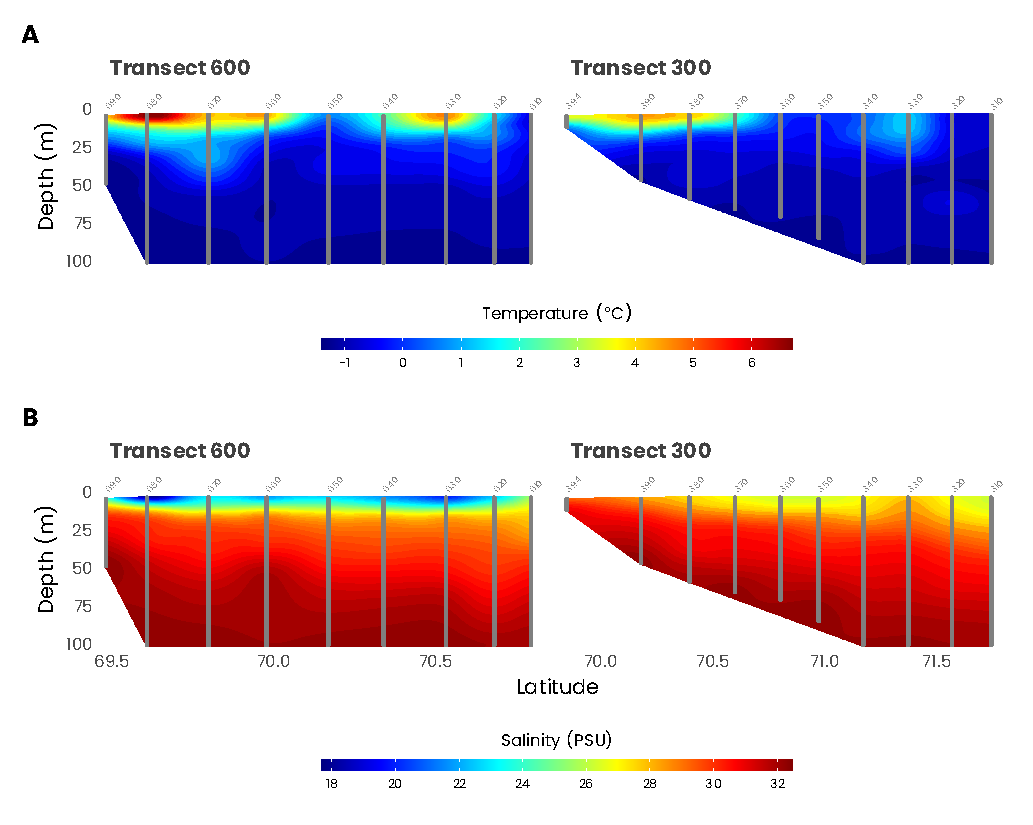
\includegraphics[scale = 0.85]{../../../graphs/fig05.pdf}
    \caption{Cross-sections of (\textbf{A}) absoprtion ($a(440)$) and (\textbf{B}) total scattering ($b_b(440)$) measured from the barge at 440 nm with an AC9 and BB9 respectively along transects 600 and 300. Station numbers are identified in light gray on top of each panel. Note that the data has been square-root transformed for the visualization.}
\end{figure}

\clearpage

\begin{figure}[H]
    \centering
    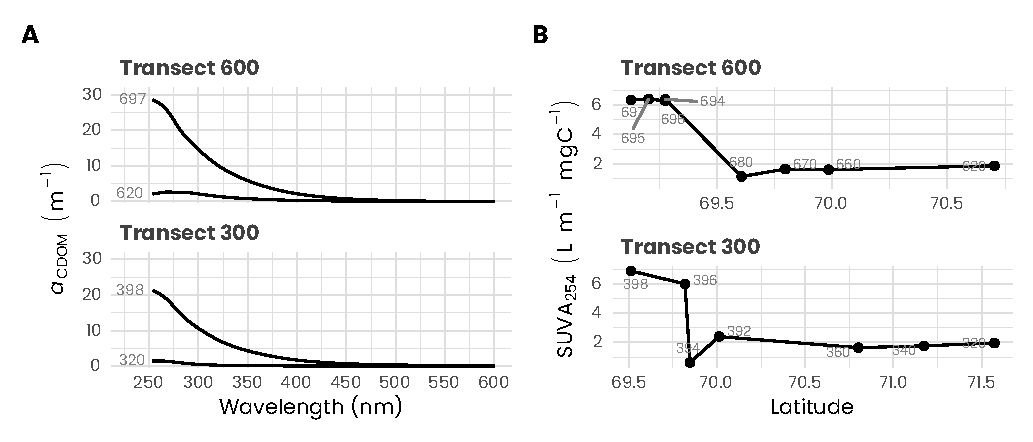
\includegraphics[scale = 0.85]{../../../graphs/fig06.pdf}
    \caption{Cross-sections of (\textbf{A}) NO$_3^-$ and (\textbf{B}) PO$_4^{3-}$ measured from Niskin bottles (gray dots) along transects 600 and 300. (\textbf{C}) N\textsuperscript{*} defined as N - rP with r = N/P = 13.1 (see the text for the details). Station numbers are identified in light gray on top of each panel.}
\end{figure}

\clearpage

\begin{figure}[H]
    \centering
    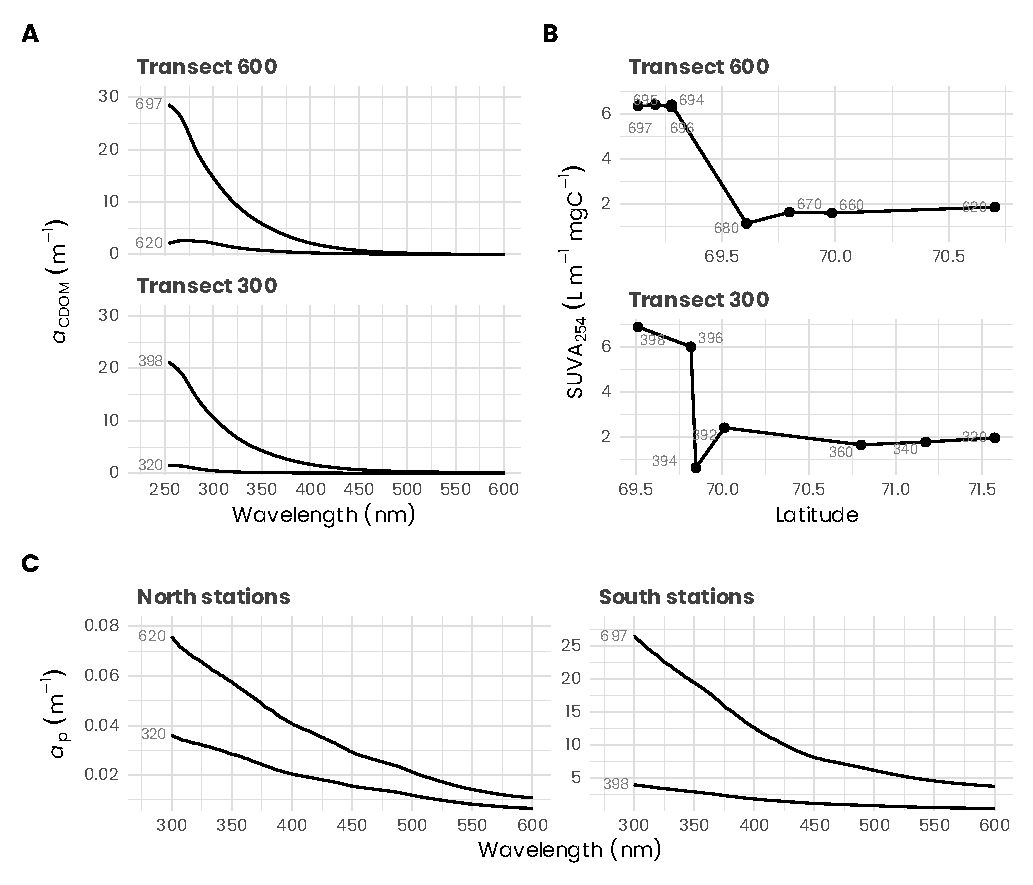
\includegraphics[scale = 1]{../../../graphs/fig07.pdf}
    \caption{(\textbf{A}) Absorption spectra between 254 and 600 nm of chromophoric dissolved organic matter ($a_{\text{CDOM}}$) measured at the surface for the northern and southern stations of the transects 600 and 300. (\textbf{B}) Specific UV absorbance at 254 nm (SUVA\textsubscript{254}, i.e. absorption of light at 254 nm per unit of carbon) at surface for stations along transects 600 and 300. Stations are identified in light gray.}
\end{figure}

\clearpage

\begin{figure}[H]
    \centering
    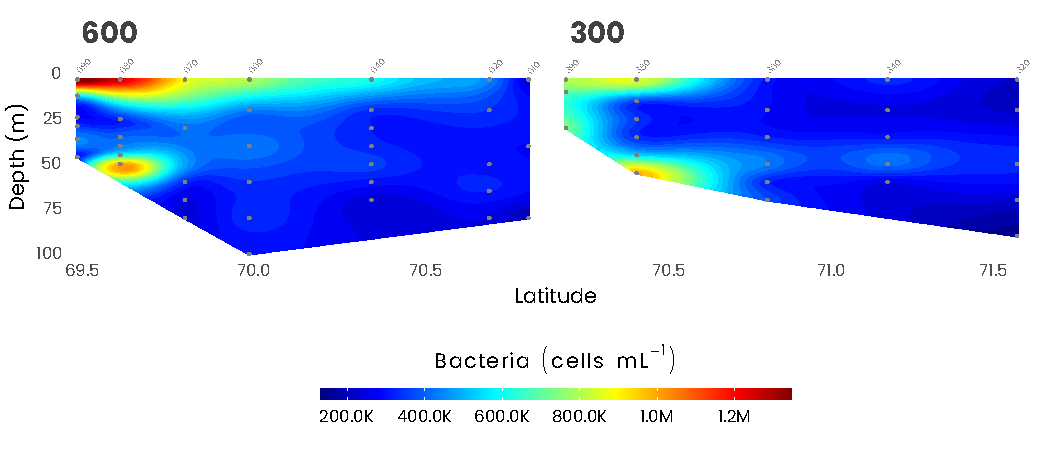
\includegraphics[scale = 1]{../../../graphs/fig08.pdf}
    \caption{Concentrations of (\textbf{A}) dissolved organic carbon (DOC), (\textbf{B}) total dissolved lignin phenols (TDLP\textsubscript{9}), and (\textbf{C}) total hydrolysable amino acids (THAA) measured along transects 600 and 300, and plotted against salinity.}
\end{figure}

\clearpage

\begin{figure}[H]
    \centering
    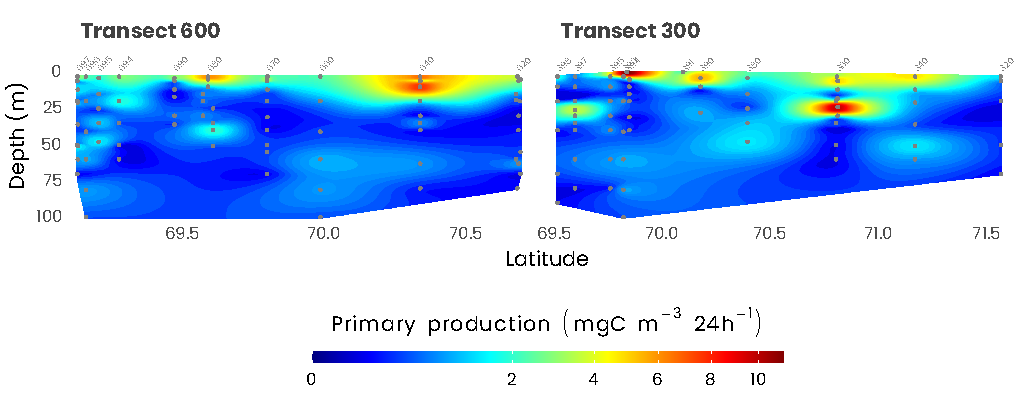
\includegraphics[scale = 1]{../../../graphs/fig09.pdf}
    \caption{Cross-sections of total chlorophyll-a measured from HPLC (gray dots) along transects 600 and 300. Station numbers are identified in light gray on top of each panel. Note that the data has been square-root transformed for the visualization.}
\end{figure}

\clearpage

\begin{figure}[H]
    \centering
    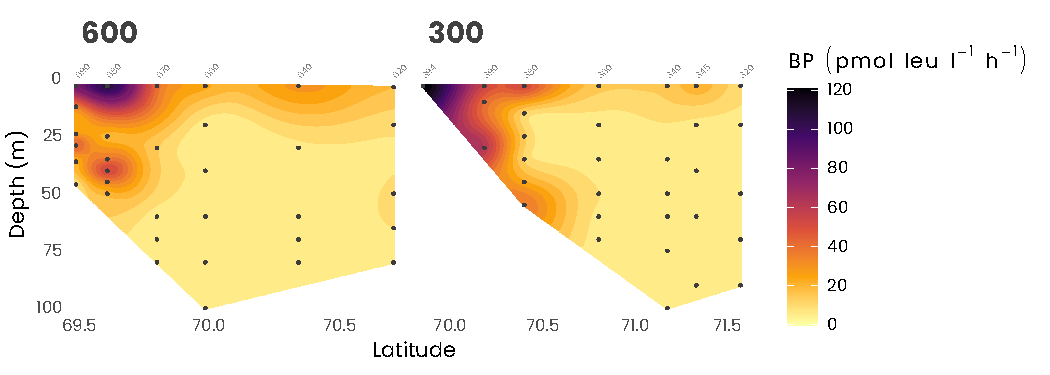
\includegraphics[scale = 1]{../../../graphs/fig10.pdf}
    \caption{Concentrations of photosynthetic (\textbf{A}) pico- and (\textbf{B}) nano-eukaryotes measured by flow cytometry during the MALINA cruise on transects 600 and 300.}
\end{figure}

\clearpage

\begin{figure}[H]
    \centering
    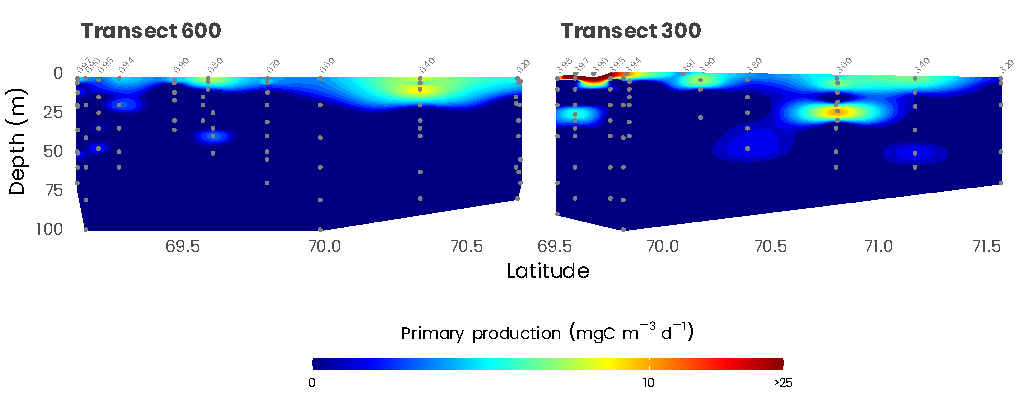
\includegraphics[scale = 1]{../../../graphs/fig11.pdf}
    \caption{(\textbf{A}) Taxonomic composition of populations of photosynthetic pico- and nano-eukaryotes sorted flow cytometry from clone library sequences  \citep{Balzano2012a}. (\textbf{B}) Taxonomic composition of cultures of phytoplankton isolated during the MALINA cruise \citep{Balzano2012b}.}
\end{figure}

\clearpage

\begin{figure}[H]
    \centering
    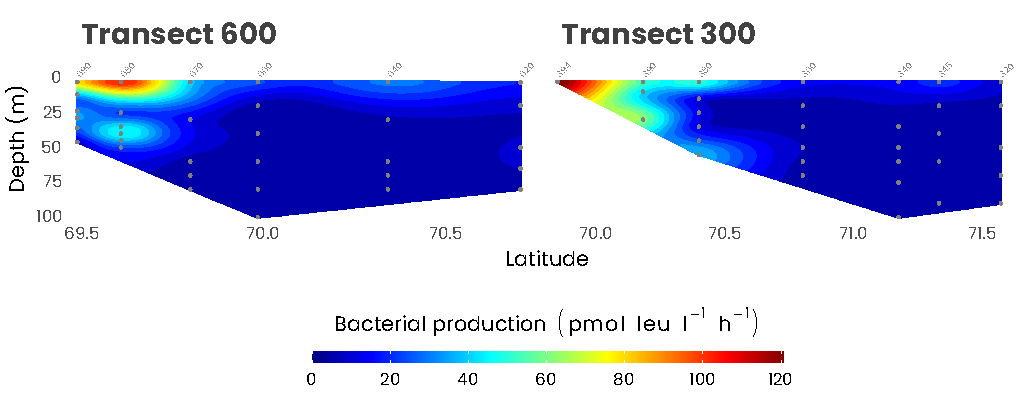
\includegraphics[scale = 1]{../../../graphs/fig12.pdf}
    \caption{Cross-sections of primary production (gray dots) along transects 600 and 300. Station numbers are identified in light gray on top of each panel. Note that the color scale is presented on a log10 scale.}
\end{figure}

\clearpage

\begin{figure}[H]
    \centering
    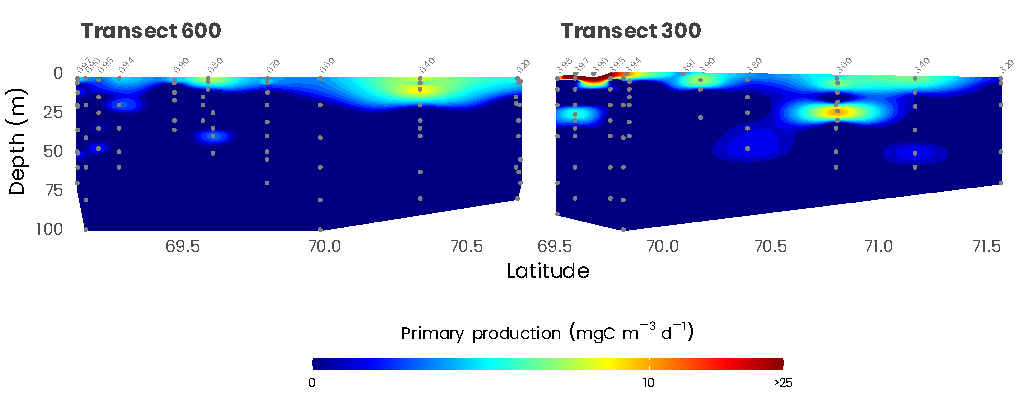
\includegraphics[scale = 1]{../../../graphs/fig13.pdf}
    \caption{(\textbf{A}) CO and CO$_2$ production measured at 295 nm at surface for stations of transects 600 and 300. (\textbf{B}) Autoxidation of suspended particulate material for stations of transects 600 and 300.}
\end{figure}

\clearpage

\begin{figure}[H]
    \centering
    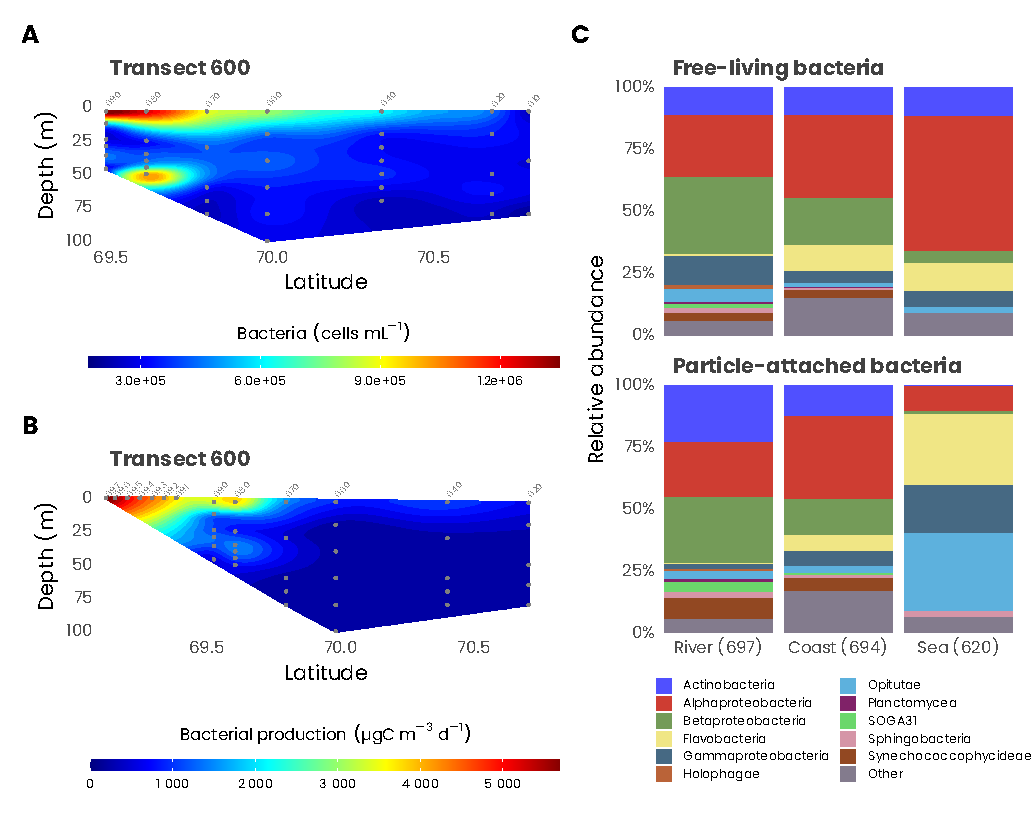
\includegraphics[scale = 1]{../../../graphs/fig14.pdf}
    \caption{(\textbf{A}) Cross-sections of bacterial abundance measured from flow cytometry and (\textbf{B}) bacterial production measured along transect 600. Station numbers are identified in light gray on top of each panel. (\textbf{C}) Cumulative bar charts comparing the relative class abundances in particle-attached (PA) and free-living (FL) for a selected number of samples in transect 600.}
\end{figure}

\begin{figure}[H]
    \centering
    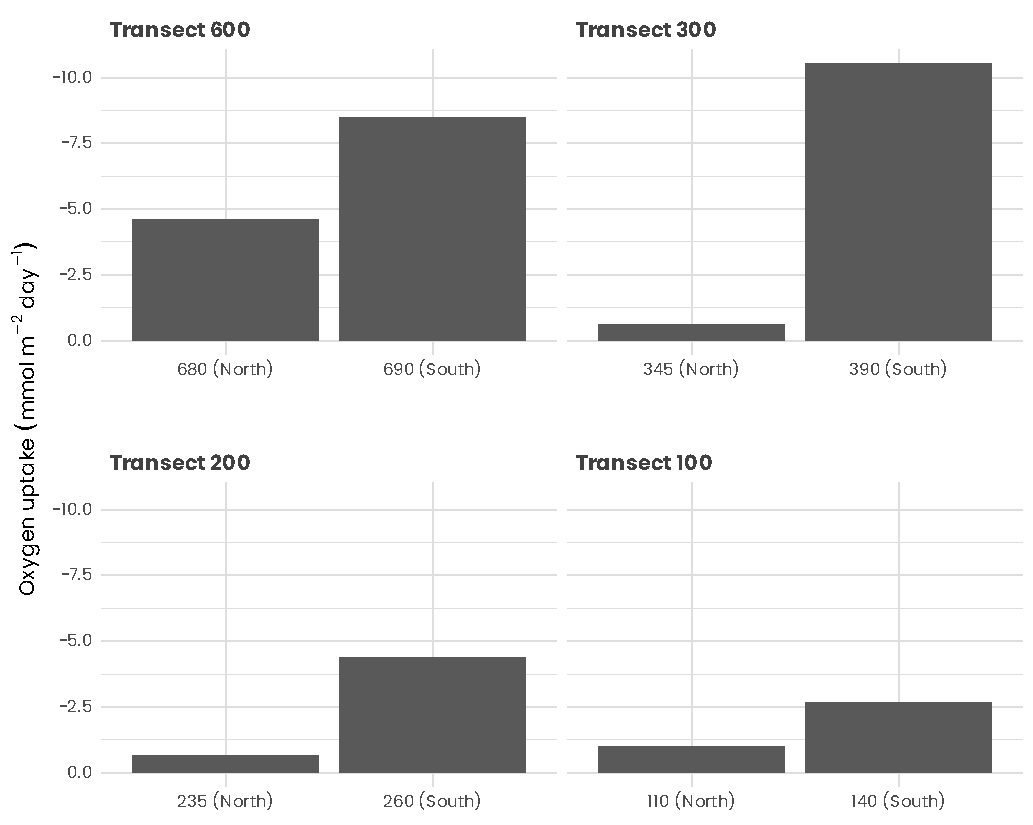
\includegraphics[scale = 1]{../../../graphs/fig_o2_uptake.pdf}
    \caption{xxx}
\end{figure}

\clearpage

\begingroup\fontsize{5}{7}\selectfont

\begin{longtable}[t]{llll}
\caption{\label{tab:}Parameters measured during the MALINA oceanographic expedition. Parameters are ordered by alphabetical order.}\\
\toprule
Parameters & Method & Sampling & Principal investigators\\
\midrule
\endfirsthead
\caption[]{Parameters measured during the MALINA oceanographic expedition. Parameters are ordered by alphabetical order. \textit{(continued)}}\\
\toprule
Parameters & Method & Sampling & Principal investigators\\
\midrule
\endhead
\
\endfoot
\bottomrule
\endlastfoot
\textsuperscript{137}Cs datation of core samples & Gamma spectrometry & Box corer & Rochon A./ Schmidt\\
\textsuperscript{137}Cs datation of core samples & Gamma spectrometer & CASQ corer & Rochon A./ Schmidt\\
\textsuperscript{14}C datation of core samples & Accelerator Mass Spectrometry & Box corer & Rochon A.\\
\textsuperscript{14}C datation of core samples & Accelerator Mass Spectrometry & CASQ corer & Rochon A.\\
\textsuperscript{15}N-Ammonium assimilation & \textsuperscript{15}N spiking - incubation - mass-spectrometry & Rosette - Deck incubations & Tremblay J.E./ Raimbault P.\\
\addlinespace
\textsuperscript{15}N-Ammonium assimilation & \textsuperscript{15}N spiking - incubation - mass-spectrometry & Rosette In-situ production line & Tremblay J.E./ Raimbault P.\\
\textsuperscript{15}N-Ammonium oxidation (Nitrification) & \textsuperscript{15}N spiking - incubation - mass-spectrometry & Rosette - Deck incubations & Tremblay J.E./ Raimbault P.\\
\textsuperscript{15}N-Ammonium oxidation (Nitrification) & \textsuperscript{15}N spiking - incubation - mass-spectrometry & Rosette In-situ production line & Tremblay J.E./ Raimbault P.\\
\textsuperscript{15}N-Ammonium primary production (\textsuperscript{13}C) & \textsuperscript{15}N spiking - incubation - mass-spectrometry & Rosette - Deck incubations & Tremblay J.E./ Raimbault P.\\
\textsuperscript{15}N-Ammonium regeneration & \textsuperscript{15}N spiking - incubation - mass-spectrometry & Rosette - Deck incubations & Tremblay J.E./ Raimbault P.\\
\addlinespace
\textsuperscript{15}N-Ammonium regeneration & \textsuperscript{15}N spiking - incubation - mass-spectrometry & Rosette In-situ production line & Tremblay J.E./ Raimbault P.\\
\textsuperscript{15}N-N\textsubscript{2} fixation & \textsuperscript{15}N spiking - incubation - mass-spectrometry & Rosette water sample & Tremblay J.E./ Raimbault P.\\
\textsuperscript{15}N-Nitrate assimilation & \textsuperscript{15}N spiking - incubation - mass-spectrometry & Rosette - Deck incubations & Tremblay J.E./ Raimbault P.\\
\textsuperscript{15}N-Nitrate assimilation & \textsuperscript{15}N spiking - incubation - mass-spectrometry & Rosette In-situ production line & Tremblay J.E./ Raimbault P.\\
\textsuperscript{15}N-Urea Photosynthetic parameters & \textsuperscript{15}N incubations mass spectrometry & Rosette Niskin water sample & Tremblay J.E.\\
\addlinespace
\textsuperscript{210}Pb geochronology of core samples & \textsuperscript{209}Po alpha spectrometry & Box corer & Rochon A.\\
\textsuperscript{210}Pb geochronology of core samples & \textsuperscript{209}Po alpha spectrometry & CASQ corer & Rochon A.\\
\textsuperscript{226}Ra (particulate) & Gamma spectrometry & Foredeck In-situ pump & Gasser B.\\
\textsuperscript{226}Ra/228Ra & Gamma spectrometry & Discrete Sample on Continuous System. & Gasser B.\\
\textsuperscript{234}Th (1 micron < particles > 70 micron) & Beta-counting & Foredeck In-situ pump & Gasser B.\\
\addlinespace
\textsuperscript{234}Th (particles > 70 micron) & Beta-counting & Foredeck In-situ pump & Gasser B.\\
\textsuperscript{234}Th (Particulate) & Beta-counting & Drifting Sediment trap & Gasser B.\\
\textsuperscript{234}Th (total) & Beta-counting & Rosette water sample & Gasser B.\\
\textsuperscript{238}U (Dissolved) & Derived parameter & Rosette water sample & Gasser B.\\
\textsuperscript{238}U (total) & Alpha-counting & Rosette water sample & Gasser B.\\
\addlinespace
AAPB (abundance) & IR microscopy, fluorimetry. FISH & Rosette water sample & Jeanthon C./ Boeuf D.\\
AAPB (abundance) & IR microscopy, fluorimetry. FISH & Zodiac water sample & Jeanthon C./ Boeuf D.\\
Absorption (particulate) & PSICAM & Barge water sample & Leymarie E.\\
Absorption (particulate) & Spectrophotometer (filters) & Barge water sample & Belanger S.\\
Absorption (particulate) & Spectrophotometer (filters) & Continuous on way & Belanger S.\\
\addlinespace
Absorption (particulate) & PSICAM & Rosette water sample & Leymarie E.\\
Absorption (particulate) & Spectrophotometer (filters) & Rosette water sample & Belanger S.\\
Absorption (particulate) & Spectrophotometer (filters) & Zodiac profiler & Belanger S.\\
Absorption (total) & PSICAM & Barge water sample & Leymarie E.\\
Absorption (total) & PSICAM & Rosette water sample & Leymarie E.\\
\addlinespace
Absorption coefficient (total) & HOBI-Labs a-sphere & Barge profiler & Wright V./ Hooker S.\\
Absorption coefficient (total) (9 wavelengths) & Wetlabs AC9 Serial\# 156 & Rosette profiler & Ehn J.\\
Absorption coefficient (total) (9 wavelengths in IR & Wetlabs AC9 Serial\# 303 & Barge profiler & Doxaran D.\\
Absorption coefficient (total) (9 wavelengths) & Wetlabs AC9 Serial\# 279 & Barge profiler & Doxaran D.\\
Air Relative Humidity & Humidity Sensor & Foredeck Meteorological Tower & Papakyriakou T.\\
\addlinespace
Alkalinity total (TA) & Potentiometry & Barge water sample & Mucci A./ Lansard B.\\
Alkalinity total (TA) & Potentiometry & Rosette & Mucci A./ Lansard B.\\
Alkalinity total (TA) & Potentiometry & Zodiac water sample & Mucci A./ Lansard B.\\
Alkanes & GC-MS & Box corer & Bouloubassi I.\\
Alkanes & GC-MS & CASQ corer & Bouloubassi I.\\
\addlinespace
Ammonium (NH$^+_4$) photo-production apparent quantum yield (AQY) & sun simulator - fluorimetry & Rosette water sample & Xie H./ Tremblay J.E.\\
Ammonium (NH$^+_4$) photo-production apparent quantum yield (AQY) & sun simulator - fluorimetry & Zodiac water sample & Xie H./ Tremblay J.E.\\
Aragonite : saturation state & Derived parameter & Barge water sample & Mucci A./ Lansard B.\\
Aragonite : saturation state & Derived parameter & Rosette water sample & Mucci A./ Lansard B.\\
Aragonite : saturation state & Derived parameter & Zodiac water sample & Mucci A./ Lansard B.\\
\addlinespace
Archaea (diversity) & CE-SSCP and DNA clone library & Rosette water sample & Joux F.\\
Attenuation coefficient (total) (9 wavelengths in IR) & Wetlabs AC9 Serial \#0303 & Barge profiler & Doxaran D.\\
Attenuation coefficient (total) (9 wavelengths) & Wetlabs AC9 Serial \#279 & Barge profiler & Doxaran D.\\
Attenuation coefficient (total) (9 wavelengths) & Wetlabs AC9 Serial \#156 & Rosette profiler & Ehn J.\\
Attenuation coefficient at 660 nm & Wetlabs (CRover) transmissometer & Drifting profiling float & Doxaran D.\\
\addlinespace
Backscattering 532 nm & Wetlabs (ECO3) backscatterometer & Drifting profiling float & Doxaran D.\\
Backscattering coefficient (3 wavelengths in IR) & Wetlabs ECO-BB3 serial \#538 & Barge profiler & Doxaran D.\\
Backscattering coefficient (3 wavelengths) & Wetlabs ECO-BB3 serial \#028 & Barge profiler & Doxaran D.\\
Backscattering coefficient (6 Wavelength) & HOBI-Labs Hydroscat-6 serial \# & Barge profiler & Wright V./ Hooker S.\\
Backscattering coefficient (8 wavelengths, spectral) & Hydroscat-6 (ser\#97074) and two a-Beta (HOBI-Labs) & Barge profiler & Reynolds R.\\
\addlinespace
Backscattering coefficient (8 wavelengths, spectral) & Hydroscat-6 (ser\#97074) and two a-Beta (HOBI-Labs) & Foredeck & Reynolds R.\\
Backscattering coefficient (9 wavelengths) & Wetlabs ECO-BB9 serial\# 274 & Rosette profiler & Ehn J.\\
Bacteria (abundance) & Flow cytometry & Rosette water sample & Vaulot D.\\
Bacteria (abundance) & Flow Cytometry & Rosette water sample & Joux F./ Ortega E.\\
Bacterial abundance & FISH-TSA & Rosette water sample & Joux F.\\
\addlinespace
Bacterial bio-volume & Epifluorescence microscopy & Rosette water sample & Joux F./ Ortega E.\\
Bacterial density (benthic) & Flow cytometry & Box corer & Link H./ Archambault P./ Chaillou G.\\
Bacterial diversity & CE-SSCP and DNA clone library & Rosette water sample & Joux F.\\
Bacterial Ecto-enzymatic activity & Spectrofluorimetry & Rosette water sample & Joux F./ Ortega E.\\
Bacterial growth (limitation by nutrients) & Leu-3H incubations - cells counts & Rosette water sample & Joux F./ Jeffrey W./ Ortega E.\\
\addlinespace
Bacterial production & Leucine-3H incorporation & Rosette water sample & Joux F./ Jeffrey W.\\
Bacterial production & Leucine-3H incorporation & Zodiac water sample & Joux F./ Jeffrey W.\\
Bacterial production (effects of DOM UV exposure on...) & Leucine-3H incorporation - cell counts & Rosette water sample & Joux F./ Jeffrey W./ Ortega E.\\
Bacterial production (effects of UV radiation) & Leucine-3H incorporation & Rosette water sample & Joux F./ Jeffrey W.\\
Bacterial respiration (whole community) & O\textsuperscript{2} consumption - Winkler - Incubations & Rosette water sample & Joux F./ Ortega E.\\
\addlinespace
Benthic ammonium flux & Incubations - Colorimetry & Box corer & Link H./ Archambault P./ Chaillou G.\\
Benthic DOC remineralisation & Incubations - wet oxidation & Box corer & Link H./ Archambault P./ Chaillou G./ Charriere B.\\
Benthic Macrofauna abundance & Microscopy & Box corer & Link H./ Archambault P./ Chaillou G.\\
Benthic Macrofauna biomass & Wet weight & Box corer & Link H./ Archambault P./ Chaillou G.\\
Benthic Macrofauna diversity & Microscopy & Box corer & Link H./ Archambault P./ Chaillou G.\\
\addlinespace
Benthic nitrate flux & Incubations - Colorimetry- Autoanalyzer & Box corer & Link H./ Archambault P./ Chaillou G.\\
Benthic nitrite flux & Incubations - Colorimetry- Autoanalyzer & Box corer & Link H./ Archambault P./ Chaillou G.\\
Benthic phosphate flux & Incubations - Colorimetry- Autoanalyzer & Box corer & Link H./ Archambault P./ Chaillou G.\\
Benthic respiration & Incubations - Optic - Oxygen probe & Box corer & Link H./ Archambault P./ Chaillou G.\\
Benthic silicic acid flux & Incubations - Colorimetry - Autoanalyzer & Box corer & Link H./ Archambault P./ Chaillou G.\\
\addlinespace
Bioturbation of sediments & Incubation with luminophores & Box corer & Link H./ Archambault P./ Chaillou G.\\
Calcite : saturation state & Derived parameter & Barge water sample & Mucci A./ Lansard B.\\
Calcite : saturation state & derived parameter & Rosette water sample & Mucci A./ Lansard B.\\
Calcite : saturation state & Derived parameter & Zodiac water sample & Mucci A./ Lansard B.\\
Campesterol, cholesterol, sistosterol and products of degrad & GC-MS & Rosette water sample & Sempere R.\\
\addlinespace
CDOM absorption & PSICAM & Barge water sample & Leymarie E.\\
CDOM absorption & Spectrophotometer & Barge water sample & Matsuoka A./ Bricaud A.\\
CDOM absorption & Spectrophotometer & Barge water sample & Wright V./ Hooker S.\\
CDOM absorption & Ultrapath & Barge water sample & Bricaud A.\\
CDOM absorption & PSICAM & Rosette water sample & Leymarie E.\\
\addlinespace
CDOM absorption & Spectrophotometer & Rosette water sample & Matsuoka A./ Bricaud A.\\
CDOM absorption & Ultrapath & Rosette water sample & Bricaud A.\\
CDOM absorption & PSICAM & Zodiac water sample & Leymarie E.\\
CDOM absorption & Spectrophotometer & Zodiac water sample & Matsuoka A./ Bricaud A.\\
CDOM absorption & Ultrapath & Zodiac water sample & Bricaud A.\\
\addlinespace
CDOM fluorescence & HOBI-Labs Hydroscat-6 ser\# HS080542 & Barge profiler & Wright V./ Hooker S.\\
CDOM fluorescence & Wetlabs WetStar WSCD & Barge profiler & Doxaran D.\\
CDOM fluorescence & Wetlabs (ECO3) fluorometer & Drifting profiling float & Doxaran D.\\
CDOM fluorescence & Haardt fluorometer & Rosette profiler & Belanger S./ Amon/ Sempere R.\\
CDOM fluorescence EEM (excitation-emission-matrix) & Spectrofluorimetry & Rosette water sample & Belanger S./ Amon/ Sempere R.\\
\addlinespace
CDOM fluorescence EEM (excitation-emission-matrix) & Spectrofluorimetry & Zodiac water sample & Belanger S./ Amon/ Sempere R.\\
Chlorophyll a and Phaeopigments (concentration) & Fluorimetry Size fractionned & Rosette water sample & Gosselin M./ Belanger S.\\
Chlorophyll a and Phaeopigments (benthic) & Fluorometric analysis & Box corer & Link H./ Archambault P./ Chaillou G.\\
Chlorophyll a fluorescence [Fchla (z)] & Chelsea Mini-Track a II fluorometer & Barge profiler & Doxaran D.\\
Chlorophyll a fluorescence [Fchla (z)] & HOBI-Labs Hydroscat-6 fluorometer & Barge profiler & Wright V./ Hooker S.\\
\addlinespace
Chlorophyll a fluorescence [Fchla (z)] & Wetlabs (ECO3) fluorometer & Drifting profiling float & Doxaran D.\\
Chlorophyll a fluorescence [Fchla (z)] & SeaPoint fluorometer & Rosette profiler & Gratton Y./ Prieur L./ Tremblay J.E.\\
CO photo-prod. apparent quantum yield for CDOM & Sun simulator - reduction gas analyzer & Rosette water sample & Xie H.\\
CO photo-prod. apparent quantum yield for CDOM & Sun simulator - reduction gas analyzer & Zodiac water sample & Xie H.\\
CO photo-prod. apparent quantum yield for particulate matter & Sun simulator - reduction gas analyzer & Rosette water sample & Xie H.\\
\addlinespace
CO photo-prod. apparent quantum yield for particulate matter & Sun simulator - reduction gas analyzer & Zodiac water sample & Xie H.\\
CO\textsuperscript{2} (atm) concentration & Infra Red & Foredeck Meteorological Tower & Papakyriakou T.\\
CO\textsuperscript{2} (seawater) concentration & Infra Red & Foredeck Meteorological Tower & Papakyriakou T.\\
CO3 2- concentrations & Derived parameter & Barge water sample & Mucci A./ Lansard B.\\
CO3 2- concentrations & Derived parameter & Rosette water sample & Mucci A./ Lansard B.\\
\addlinespace
CO3 2- concentrations & Derived parameter & Zodiac water sample & Mucci A./ Lansard B.\\
Coccolithophorids & Microscopy & Rosette water sample & Coupel P.\\
Conductivity (z) & Sensor on SBE Fascat CTD serial \# & Barge profiler & Doxaran D.\\
Conductivity (z) & Sensor on SBE Fascat CTD serial \# & Barge profiler & Wright V./ Hooker S.\\
Conductivity (z) & Sensor SeaBird 4c on CTD SBE-911 & Rosette profiler & Gratton Y./ Prieur L.\\
\addlinespace
CTD & Seabird & Drifting profiling float & Doxaran D.\\
Cultures of sorted populations & Sorted by flow cytometry, serial dilution and single cell pipetting & Rosette water sample & Vaulot D.\\
Current Profile [U (z)] & ADCP (LADCP) RD Instrument 300 KHz & Rosette profiler & Marec C./ Gratton Y./ Prieur L.\\
delta \textsuperscript{13}C & Mass Spectrometry & Zodiac water sample & Mucci A./ Lansard B.\\
delta \textsuperscript{13}C on suspended particulate matter & Mass Spectrometry & Rosette water sample & Tremblay J.E./ Raimbault P.\\
\addlinespace
delta \textsuperscript{15}C on suspended particulate matter & Mass Spectrometry & Rosette water sample & Tremblay J.E./ Raimbault P.\\
delta \textsuperscript{18}O - water & Mass Spectrometry & Rosette water sample & Mucci A./ Lansard B.\\
delta \textsuperscript{18}O - water & Mass Spectrometry & Zodiac water sample & Mucci A./ Lansard B.\\
delta\textsuperscript{13}C & Mass Spectrometer & Barge water sample & Mucci A./ Lansard B.\\
delta\textsuperscript{13}C & Mass Spectrometry & Rosette water sample & Mucci A./ Lansard B.\\
\addlinespace
delta\textsuperscript{18}O - water & Mass Spectrometry & Barge water sample & Mucci A./ Lansard B.\\
Diacids composition & GC/MS & Rosette water sample & Sempere R.\\
Diacids composition & GC/MS & Zodiac water sample & Sempere R.\\
Diacids photo-production apparent quantum yield (AQY) & Sun simulator - GC/MS & Zodiac water sample & Sempere R.\\
Dinoflagellates cysts Abundance & Microscopy & Box corer & Rochon A.\\
\addlinespace
Dinoflagellates cysts Abundance & Microscopy & CASQ corer & Rochon A.\\
Dinoflagellates cysts Identification & Microscopy & Box corer & Rochon A.\\
Dinoflagellates cysts Identification & Microscopy & CASQ corer & Rochon A.\\
Dissolved Inorg. Carbon photo-prod. apparent quantum yield & Sun simulator - indrared CO\textsuperscript{2} analyzer & Rosette water sample & Xie H./ Belanger S.\\
Dissolved Inorg. Carbon photo-prod. apparent quantum yield & Sun simulator - indrared CO\textsuperscript{2} analyzer & Zodiac water sample & Xie H./ Belanger S.\\
\addlinespace
Dissolved Organic Carbon (DOC) & High Temperature Catalytic Oxidation & Barge water sample & Wright V./ Hooker S.\\
Dissolved Organic Carbon (DOC) & High Temperature Catalytic Oxidation & Rosette water sample & Sempere R.\\
Dissolved Organic Carbon (DOC) & High Temperature Catalytic Oxidation & Rosette water sample & Benner R.\\
Dissolved Organic Carbon (DOC) & Wet oxidation & Rosette water sample & Tremblay J.E./ Raimbault P.\\
Dissolved Organic Carbon (DOC) & High Temperature Catalytic Oxidation & Zodiac water sample & Sempere R.\\
\addlinespace
Dissolved Organic Carbon (DOC) & High Temperature Catalytic Oxidation & Zodiac water sample & Benner R.\\
Dissolved Organic Nitrogen (DON) & Wet oxidation & Rosette water sample & Tremblay J.E./ Raimbault P.\\
Dissolved Organic Nitrogen (Total) (TDON) & High Temperature Catalytic Oxidation & Rosette water sample & Benner R.\\
Dissolved Organic Nitrogen (Total) (TDON) & High Temperature Catalytic Oxidation & Zodiac water sample & Benner R.\\
Dissolved Organic Phosphorus (DOP) & Wet oxidation & Rosette water sample & Tremblay J.E./ Raimbault P.\\
\addlinespace
Ed, Lu, Eu, Es & C-OPS package (320, 340, 380, 395 nm) & Barge profiler & Hooker\\
Electric resistivity (sediment core physical properties) & Geotek Multi Sensor Core Logger & Box corer & Rochon A.\\
Electric resistivity (sediment core physical properties) & Geotek Multi Sensor Core Logger & CASQ corer & Rochon A.\\
Eukaryotes (abundance) & DAPI epifluorescence microscopy & Rosette water sample & Lovejoy C.\\
Eukaryotes (abundance) & FISH-TSA & Rosette water sample & Lovejoy C.\\
\addlinespace
Eukaryotes (biomass) & DAPI epifluorescence microscopy & Rosette water sample & Lovejoy C.\\
fCO\textsuperscript{2} & Derived parameter & Barge water sample & Mucci A./ Lansard B.\\
fCO\textsuperscript{2} & Derived parameter & Rosette water sample & Mucci A./ Lansard B.\\
fCO\textsuperscript{2} & Derived parameter & Zodiac water sample & Mucci A./ Lansard B.\\
Foraminifera abundance & Microscopy & Box corer & Rochon A.\\
\addlinespace
Foraminifera abundance & Microscopy & CASQ corer & Rochon A.\\
Foraminifera identification & Microscopy & Box corer & Rochon A.\\
Foraminifera identification & Microscopy & CASQ corer & Rochon A.\\
Gamma density (sediment core physical properties) & Geotek Multi Sensor Core Logger & Box corer & Rochon A.\\
Gamma density (sediment core physical properties) & Geotek Multi Sensor Core Logger & CASQ corer & Rochon A.\\
\addlinespace
H\textsubscript{2}O (atm) concentration & Infrared gas analyzer & Foredeck Meteorological Tower & Papakyriakou T.\\
HCO\textsuperscript{2}- concentration & Derived parameter & Barge water sample & Mucci A./ Lansard B.\\
HCO\textsuperscript{2}- concentration & Derived parameter & Rosette water sample & Mucci A./ Lansard B.\\
HCO\textsuperscript{2}- concentration & Derived parameter & Zodiac water sample & Mucci A./ Lansard B.\\
Hydro SCAMP (Temp, Salin, Chlorophyll, turb. ...) & SCAMP profiler & In-water profiler & Gratton Y.\\
\addlinespace
Hydrolysable Amino Acids (Total) (THAA) & HPLC & Rosette water sample & Benner R.\\
Hydrolysable Amino Acids (Total) (THAA) & HPLC & Zodiac water sample & Benner R.\\
Hydroxyl radicals (OH) & HPLC & Rosette water sample & Sempere R.\\
Hydroxyl radicals (OH) & HPLC & Zodiac water sample & Sempere R.\\
Hydroxyl radicals (OH) photo-prod. apparent quantum yield & Sun simulator - HPLC & Rosette water sample & Sempere R.\\
\addlinespace
Hydroxyl radicals (OH) photo-prod. apparent quantum yield & Sun simulator - HPLC & Zodiac water sample & Sempere R.\\
IP25 (C25 Monounsaturated Hydrocarbon) & GC & Box corer & Masse G.\\
IP25 (C25 Monounsaturated Hydrocarbon) & GC & CASQ corer & Masse G.\\
Irradiance & Satlantic (PUV) (305,325, 340, 380,..) & Foredeck & Sempere R.\\
Irradiance (412, 490, 555 nm) & Satlantic (OCR) radiometer & Drifting profiling float & Doxaran D.\\
\addlinespace
Lignin phenols (dissolved) & GC/MS & Rosette water sample & Benner R.\\
Lignin phenols (dissolved) & GC/MS & Zodiac water sample & Benner R.\\
Lipid biomarqueurs & GC-Flamme Ionization Detection / GC-MS & Box corer & Tolosa I.\\
Lipid biomarqueurs & GC-Flamme Ionization Detection / GC-MS & CASQ corer & Tolosa I.\\
Lipid biomarqueurs d\textsuperscript{13}C & GC-Combustion Isotope ratio MS & Box corer & Tolosa I.\\
\addlinespace
Lipid biomarqueurs d\textsuperscript{13}C & GC-Combustion Isotope ratio MS & CASQ corer & Tolosa I.\\
Long-Wave radiation (Lwin) & Pyrgeometer & Wheel-house radiation platform & Papakyriakou T.\\
Magnetic susceptibility (sediment core physical properties) & Geotek Multi Sensor Core Logger & Box corer & Rochon A.\\
Magnetic susceptibility (sediment core physical properties) & Geotek Multi Sensor Core Logger & CASQ corer & Rochon A.\\
Nanoeukaryotes (abundance) & Flow cytometry & Rosette water sample & Vaulot D.\\
\addlinespace
NH$^+_4$ & Fluorescence & Rosette water sample & Tremblay J.E./ Raimbault P.\\
Nitrate (concentration) & Satlantic ISUS & Rosette profiler & Gratton Y./ Prieur L./ Tremblay J.E.\\
NO$^-_2$ & Colorimetry/Autoanalyzer & Rosette water sample & Tremblay J.E./ Raimbault P.\\
NO$^-_3$ & Colorimetry/Autoanalyzer & Rosette water sample & Tremblay J.E./ Raimbault P.\\
Organic Compounds High Molecular Weight (HMW) & Sun simulator incubations - HPLC & Rosette water sample & Xie H.\\
\addlinespace
Organic Compounds High Molecular Weight (HMW) & Sun simulator incubations - HPLC & Zodiac water sample & Xie H.\\
Organic Compounds Low Molecular Weight (LMW) & Sun simulator incubations - HPLC & Rosette water sample & Xie H.\\
Organic Compounds Low Molecular Weight (LMW) & Sun simulator incubations - HPLC & Zodiac water sample & Xie H.\\
Oxygen (dissolved) & Discrete samples Winkler Method & Barge water sample & Prieur L.\\
Oxygen (dissolved) & Idronaut Ocean Seven O\textsuperscript{2} sensor & Continuous horizontal & Papakyriakou T.\\
\addlinespace
Oxygen (dissolved) & SeaBird SBE-43 sensor & Rosette profiler & Gratton Y./ Prieur L.\\
Oxygen (dissolved) & Discrete samples Winkler Method & Rosette water sample & Prieur L.\\
Oxygen (dissolved) & Discrete samples Winkler Method & Zodiac water sample & Prieur L.\\
P waves speed (sediment core physical properties) & Geotek Multi Sensor Core Logger & Box corer & Rochon A.\\
P waves speed (sediment core physical properties) & Geotek Multi Sensor Core Logger & CASQ corer & Rochon A.\\
\addlinespace
Paleomagnetism & Cryogenic magnetometer & Box corer & Rochon A.\\
Paleomagnetism & Cryogenic magnetometer & CASQ corer & Rochon A.\\
PAR & Biospherical sensor & Barge profiler & Wright V./ Hooker S.\\
PAR & Biospherical sensor & Rosette profiler & Gratton Y./ Prieur L./ Tremblay J.E.\\
PAR & PARLite sensor & Wheel-house radiation platform & Papakyriakou T.\\
\addlinespace
Particle Size Distribution & LISST-100X & Barge profiler & Reynolds R.\\
Particle Size Distribution & Coulter counter & Barge water sample & Reynolds R.\\
Particle Size Distribution & UVP-5 & In-water profiler & Picheral M.\\
Particle Size Distribution & LISST-100X & Rosette profiler & Reynolds R.\\
Particle Size Ditribution & Coulter counter & Rosette water sample & Reynolds R.\\
\addlinespace
Particulate Organic Carbon (POC) & CHN analyzer & Barge water sample & Wright V./ Hooker S.\\
Particulate Organic Carbon (POC) & CHN analyzer on SPM filters & Barge water sample & Doxaran D./ Ehn J./ Babin M.\\
Particulate Organic Carbon (POC) & CHN analyzer on SPM filters & Rosette water sample & Doxaran D./ Ehn J./ Babin M.\\
Particulate Organic Carbon (POC) & Wet oxidation & Rosette water sample & Tremblay J.E./ Raimbault P.\\
Particulate Organic Carbon (POC) & CHN analyzer on SPM filters & Zodiac water sample & Doxaran D./ Ehn J./ Babin M.\\
\addlinespace
Particulate Organic Matter (POM) & CHN analyzer on SPM filters & Barge water sample & Wright V./ Hooker S.\\
Particulate Organic Nitrogen (PON) & CHN analyzer & Barge water sample & Wright V./ Hooker S.\\
Particulate Organic Nitrogen (PON) & Wet oxidation & Rosette water sample & Tremblay J.E./ Raimbault P.\\
Particulate Organic Phosphorus (POP) & Wet oxidation & Rosette water sample & Tremblay J.E./ Raimbault P.\\
pH & Spectrophometry & Barge water sample & Mucci A./ Lansard B.\\
\addlinespace
pH & SeaBird SBE-18 sensor & Rosette profiler & Gratton Y./ Prieur L./ Tremblay J.E.\\
pH & Spectrophotometry & Rosette water sample & Mucci A./ Lansard B.\\
pH & Spectrophometry & Zodiac water sample & Mucci A./ Lansard B.\\
pH (total proton scale) & Derived parameter & Barge water sample & Mucci A./ Lansard B.\\
pH (total proton scale) & Dervide parameter & Rosette water sample & Mucci A./ Lansard B.\\
\addlinespace
pH (total proton scale) & Dervide parameter & Zodiac water sample & Mucci A./ Lansard B.\\
Photosynthetic eukaryotes (morphology) & Scanning Electron Microscopy & Rosette water sample & Vaulot D.\\
Photosynthetic  eukaryotes (diversity) & DNA clone library and TRFLP of sorted populations & Rosette water sample & Vaulot D.\\
Photoheterotrophs (diel cycle genes analyses) & RNA expression every 4 hours & Rosette water sample & Jeanthon C./ Boeuf D.\\
Photoheterotrophs (DNA diversity) & DNA clone library & Rosette water sample & Jeanthon C./ Boeuf D.\\
\addlinespace
Photoheterotrophs (metagenome) & 454 sequencing & Rosette water sample & Jeanthon C./ Boeuf D.\\
Photosynthetic parameters & \textsuperscript{14}C incubations & Rosette water sample & Huot Y.\\
Phytoplankton (abundance) & Inverted microscope & Rosette water sample & Gosselin M./ Belanger S.\\
Phytoplankton (taxonomy) & Inverted microscope & Rosette water sample & Gosselin M./ Belanger S.\\
Phytoplankton pigments & HPLC & Barge water sample & Wright V./ Hooker S.\\
\addlinespace
Phytoplankton pigments & HPLC & Rosette water sample & Ras J./ Claustre H.\\
Picoeukaryotes (abundance) & Flow cytometry & Rosette water sample & Vaulot D.\\
Picoplankton (diversity) & DNA clone library & Rosette water sample & Lovejoy C.\\
Photosynthetic  eukaryotes (diversity) & DNA from filters & Rosette water sample & Vaulot D.\\
Picoplankton (diversity) & RNA clone library & Rosette water sample & Lovejoy C.\\
\addlinespace
Plankton taxonomy & UVP-5 & In-water profiler & Picheral M./ Marec C.\\
(PO$_4)^{3-}$ & Colorimetry/Autoanalyzer & Rosette water sample & Tremblay J.E./ Raimbault P.\\
Pollen and Spores Abundance & Microscopy & Box corer & Rochon A.\\
Pollen and Spores Abundance & Microscopy & CASQ corer & Rochon A.\\
Pollen and Spores Identification & Microscopy & Box corer & Rochon A.\\
\addlinespace
Pollen and Spores Identification & Microscopy & CASQ corer & Rochon A.\\
PR-containing bacteria (abundance) & Q-PCR & Rosette water sample & Jeanthon C./ Boeuf D.\\
Pressure (Barometric) & Pressure Sensor & Foredeck Meteorological Tower & Papakyriakou T.\\
Radiance & Camera Luminance & Profile mode & Antoine D./ Leymarie E.\\
Radiance & Camera Luminance & Surface mode & Antoine D./ Leymarie E.\\
\addlinespace
Radiance (surface leaving radiance) & BIO-SHADE & Barge profiler & Hooker\\
Radiance (surface leaving radiance) & BIOSORS & Foredeck & Hooker\\
Radiance (surface leaving radiance) & Satlantic HyperSAS & Foredeck & Belanger S.\\
Radiance (surface leaving radiance) & TriOS above water sensor & Foredeck & Doxaran D.\\
Radiance : Sub Product : average cosines & Camera Luminence & Profile mode & Antoine D./ Leymarie E.\\
\addlinespace
Radiance : Sub Product : average cosines & Camera Luminence & Surface mode & Antoine D./ Leymarie E.\\
Radiance : Sub Product : irradiance (E) & Camera Luminence & Profile mode & Antoine D./ Leymarie E.\\
Radiance : Sub Product : irradiance (E) & Camera Luminence & Surface mode & Antoine D./ Leymarie E.\\
Radiance : Sub Product : Lnadir & Camera Luminence & Profile mode & Antoine D./ Leymarie E.\\
Radiance : Sub Product : Lnadir & Camera Luminence & Surface mode & Antoine D./ Leymarie E.\\
\addlinespace
Radiance : Sub Product : Qnadir & Camera Luminence & Profile mode & Antoine D./ Leymarie E.\\
Radiance : Sub Product : Qnadir & Camera Luminence & Surface mode & Antoine D./ Leymarie E.\\
Radiance : Sub Product : scalar irradiance (Escal) & Camera Luminence & Profile mode & Antoine D./ Leymarie E.\\
Radiance : Sub Product : scalar irradiance (Escal) & Camera Luminence & Surface mode & Antoine D./ Leymarie E.\\
Rotational movement (accx, accy, accz,rx,ry,rz) & multi-axis inertial sensing system & Foredeck Meteorological Tower & Papakyriakou T.\\
\addlinespace
Salinity & Salinometer & Barge water sample & Gratton Y./ Prieur L.\\
Salinity & Salinometer & Rosette water sample & Gratton Y./ Prieur L.\\
Salinity (sea surface) SSS & Thermosalinograph - underway system & Continuous horizontal & Papakyriakou T.\\
Salinity [S (z)] & Derived parameter from SBE Fastcat LOC IOP pack. & Barge profiler & Doxaran D.\\
Salinity [S (z)] & Derived parameter from SBE Fastcat NASA IOP pack. & Barge profiler & Wright V./ Hooker S.\\
\addlinespace
Salinity [S (z)] & Derived parameter & Rosette profiler & Gratton Y./ Prieur L./ Tremblay J.E.\\
Short-Wave radiation (Swin) & Pyranometer & Wheel-house radiation platform & Papakyriakou T.\\
Si (OH)\textsubscript{4} & Colorimetry/Autoanalyzer & Rosette water sample & Tremblay J.E./ Raimbault P.\\
SPM (Suspended Particulate Material) & dry weight (gravimetry) & Barge water sample & Wright V./ Hooker S.\\
SPM (Suspended Particulate Material) & dry weight (gravimetry) & Barge water sample & Doxaran D./ Ehn J./ Babin M.\\
\addlinespace
SPM (Suspended Particulate Material) & dry weight (gravimetry) & Rosette water sample & Doxaran D./ Ehn J./ Babin M.\\
SPM (Suspended Particulate Material) & dry weight (gravimetry) & Zodiac water sample & Doxaran D./ Ehn J./ Babin M.\\
Sugars & HPLC & Rosette water sample & Sempere R.\\
Sugars & HPLC & Zodiac water sample & Sempere R.\\
Synechococcus (abundance) & Flow cytometry & Rosette water sample & Vaulot D.\\
\addlinespace
Temperature (Air) & Temperature Sensor & Foredeck Meteorological Tower & Papakyriakou T.\\
Temperature (Sea Surface) & Thermosalinograph - underway system & Continuous horizontal & Papakyriakou T.\\
Temperature (Surface Skin) & IR transducer & Foredeck Meteorological Tower & Papakyriakou T.\\
Temperature [T (z)] & Temp sensor on SBE Fastcat CTD serial \# & Barge profiler & Doxaran D.\\
Temperature [T (z)] & Temp sensor on SBE Fastcat CTD serial \# & Barge profiler & Wright V./ Hooker S.\\
\addlinespace
Temperature [T (z)] & Sensor SeaBird 3plus on CTD SBE-911 & Rosette profiler & Gratton Y./ Prieur L./ Tremblay J.E.\\
Total Inorganic Carbon (TIC) & Derived parameter & Barge water sample & Mucci A./ Lansard B.\\
Total Inorganic Carbon (TIC) & Derived parameter & Rosette water sample & Mucci A./ Lansard B.\\
Total Inorganic Carbon (TIC) & Derived parameter & Zodiac water sample & Mucci A./ Lansard B.\\
Total Organic Carbon (TOC) & Wet oxidation & Rosette water sample & Tremblay J.E./ Raimbault P.\\
\addlinespace
Total Organic Nitrogen (TON) & Wet oxidation & Rosette water sample & Tremblay J.E./ Raimbault P.\\
Total Organic Phosphorus (TOP) & Wet oxidation & Rosette water sample & Tremblay J.E./ Raimbault P.\\
Trace metals & X-Ray fluorescence spectroscopy & Box corer & Martinez P.\\
Trace metals & X-Ray fluorescence spectroscopy & CASQ corer & Martinez P.\\
Urea (concentration) & Spectrophotometry & Rosette water sample & Tremblay J.E./ Raimbault P.\\
\addlinespace
Volume Scattering Function (VSF) & Benchtop use of POLVSM & Barge water sample & Chami M.\\
Volume Scattering Function (VSF) & Benchtop use of POLVSM & Rosette water sample & Chami M.\\
Volume Scattering Function (VSF) & Benchtop use of POLVSM & Zodiac water sample & Chami M.\\
Wind direction & Vane & Foredeck Meteorological Tower & Papakyriakou T.\\
Wind speed & Anemometer & Foredeck Meteorological Tower & Papakyriakou T.\\
\addlinespace
Major and minor elements & XRF core scanner & CASQ corer & Martinez P.\\*
\end{longtable}
\endgroup{}


%% The following commands are for the statements about the availability of data sets and/or software code corresponding to the manuscript.
%% It is strongly recommended to make use of these sections in case data sets and/or software code have been part of your research the article is based on.

\codedataavailability{TODO} %% use this section when having data sets and software code available

\appendix


\noappendix       %% use this to mark the end of the appendix section

%% Regarding figures and tables in appendices, the following two options are possible depending on your general handling of figures and tables in the manuscript environment:

%% Option 1: If you sorted all figures and tables into the sections of the text, please also sort the appendix figures and appendix tables into the respective appendix sections.
%% They will be correctly named automatically.

%% Option 2: If you put all figures after the reference list, please insert appendix tables and figures after the normal tables and figures.
%% To rename them correctly to A1, A2, etc., please add the following commands in front of them:

\appendixfigures  %% needs to be added in front of appendix figures

\appendixtables   %% needs to be added in front of appendix tables

%% Please add \clearpage between each table and/or figure. Further guidelines on figures and tables can be found below.

\authorcontribution{} %% this section is mandatory for the journals ACP and GMD. For all other journals it is strongly recommended to make use of this section

\competinginterests{The authos declar no competing interests.} %% this section is mandatory even if you declare that no competing interests are present

\begin{acknowledgements}
    This work is dedicated to the memory of Captain Marc Thibault (commanding officer of the CCGS Amundsen, Canadian Coast Guard), Daniel Dubé (CCGS Amundsen helicopter pilot, Transport Canada) and Dr. Klaus Hochheim (research scientist at the Centre for Earth Observation Science, University of Manitoba) who died in the CCGS Amundsen helicopter crash on the evening of 09/09/13 in the icy waters of McClure Strait in the Canadian Arctic. We are very grateful to the captain (Marc Thibault) and crews of the Canadian research icebreaker CCGS Amundsen during the Malina cruise in the Beaufort Sea. This study was conducted as part of the Malina scientific program funded by ANR (Agence Nationale de la Recherche), INSU-CNRS (Institut National des Sciences de l’Univers - Centre National de la Recherche Scientifique), CNES (Centre National d'Études Spatiales) and ESA (European Space Agency). The International Atomic Energy Agency is grateful to the Government of the Principality of Monaco for the support provided to its Environment Laboratories.
\end{acknowledgements}


%% Since the Copernicus LaTeX package includes the BibTeX style file copernicus.bst,
%% authors experienced with BibTeX only have to include the following two lines:
%%
\bibliographystyle{copernicus}
\bibliography{/home/filoche/Documents/library.bib}
%%
%% URLs and DOIs can be entered in your BibTeX file as:
%%
%% URL = {http://www.xyz.org/~jones/idx_g.htm}
%% DOI = {10.5194/xyz}


%% LITERATURE CITATIONS
%%
%% command                        & example result
%% \citet{jones90}|               & Jones et al. (1990)
%% \citep{jones90}|               & (Jones et al., 1990)
%% \citep{jones90,jones93}|       & (Jones et al., 1990, 1993)
%% \citep[p.~32]{jones90}|        & (Jones et al., 1990, p.~32)
%% \citep[e.g.,][]{jones90}|      & (e.g., Jones et al., 1990)
%% \citep[e.g.,][p.~32]{jones90}| & (e.g., Jones et al., 1990, p.~32)
%% \citeauthor{jones90}|          & Jones et al.
%% \citeyear{jones90}|            & 1990



%% FIGURES

%% When figures and tables are placed at the end of the MS (article in one-column style), please add \clearpage
%% between bibliography and first table and/or figure as well as between each table and/or figure.


%% ONE-COLUMN FIGURES

%%f
%\begin{figure}[t]
%\includegraphics[width=8.3cm]{FILE NAME}
%\caption{TEXT}
%\end{figure}
%
%%% TWO-COLUMN FIGURES
%
%%f
%\begin{figure*}[t]
%\includegraphics[width=12cm]{FILE NAME}
%\caption{TEXT}
%\end{figure*}
%
%
%%% TABLES
%%%
%%% The different columns must be seperated with a & command and should
%%% end with \\ to identify the column brake.
%
%%% ONE-COLUMN TABLE
%
%%t
%\begin{table}[t]
%\caption{TEXT}
%\begin{tabular}{column = lcr}
%\tophline
%
%\middlehline
%
%\bottomhline
%\end{tabular}
%\belowtable{} % Table Footnotes
%\end{table}
%
%%% TWO-COLUMN TABLE
%
%%t
%\begin{table*}[t]
%\caption{TEXT}
%\begin{tabular}{column = lcr}
%\tophline
%
%\middlehline
%
%\bottomhline
%\end{tabular}
%\belowtable{} % Table Footnotes
%\end{table*}
%
%%% LANDSCAPE TABLE
%
%%t
%\begin{sidewaystable*}[t]
%\caption{TEXT}
%\begin{tabular}{column = lcr}
%\tophline
%
%\middlehline
%
%\bottomhline
%\end{tabular}
%\belowtable{} % Table Footnotes
%\end{sidewaystable*}
%
%
%%% MATHEMATICAL EXPRESSIONS
%
%%% All papers typeset by Copernicus Publications follow the math typesetting regulations
%%% given by the IUPAC Green Book (IUPAC: Quantities, Units and Symbols in Physical Chemistry,
%%% 2nd Edn., Blackwell Science, available at: http://old.iupac.org/publications/books/gbook/green_book_2ed.pdf, 1993).
%%%
%%% Physical quantities/variables are typeset in italic font (t for time, T for Temperature)
%%% Indices which are not defined are typeset in italic font (x, y, z, a, b, c)
%%% Items/objects which are defined are typeset in roman font (Car A, Car B)
%%% Descriptions/specifications which are defined by itself are typeset in roman font (abs, rel, ref, tot, net, ice)
%%% Abbreviations from 2 letters are typeset in roman font (RH, LAI)
%%% Vectors are identified in bold italic font using \vec{x}
%%% Matrices are identified in bold roman font
%%% Multiplication signs are typeset using the LaTeX commands \times (for vector products, grids, and exponential notations) or \cdot
%%% The character * should not be applied as mutliplication sign
%
%
%%% EQUATIONS
%
%%% Single-row equation
%
%\begin{equation}
%
%\end{equation}
%
%%% Multiline equation
%
%\begin{align}
%& 3 + 5 = 8\\
%& 3 + 5 = 8\\
%& 3 + 5 = 8
%\end{align}
%
%
%%% MATRICES
%
%\begin{matrix}
%x & y & z\\
%x & y & z\\
%x & y & z\\
%\end{matrix}
%
%
%%% ALGORITHM
%
%\begin{algorithm}
%\caption{...}
%\label{a1}
%\begin{algorithmic}
%...
%\end{algorithmic}
%\end{algorithm}
%
%
%%% CHEMICAL FORMULAS AND REACTIONS
%
%%% For formulas embedded in the text, please use \chem{}
%
%%% The reaction environment creates labels including the letter R, i.e. (R1), (R2), etc.
%
%\begin{reaction}
%%% \rightarrow should be used for normal (one-way) chemical reactions
%%% \rightleftharpoons should be used for equilibria
%%% \leftrightarrow should be used for resonance structures
%\end{reaction}
%
%
%%% PHYSICAL UNITS
%%%
%%% Please use \unit{} and apply the exponential notation


\end{document}
